\documentclass{article}
\usepackage[spanish]{babel}
\usepackage[utf8x]{inputenc}
\usepackage{graphicx}
\usepackage{epstopdf}
\epstopdfsetup{outdir=./}
\usepackage{hyperref}
\usepackage{fourier}
\usepackage{amsmath}
\usepackage{booktabs}
\usepackage[inline]{enumitem}
% colors for hyperlinks
% colored borders (false) colored text (true)
\hypersetup{colorlinks=true,citecolor=black,filecolor=black,linkcolor=black,urlcolor=black}

% package for bibliography
\usepackage[authoryear,round]{natbib}
\renewcommand{\baselinestretch}{1.2} 

% package for header
% \usepackage[automark]{scrpage2}
% \pagestyle{scrheadings}
% \ihead[]{Rafael Pérez Torres}
% \ohead[]{\today}
% \cfoot[]{\pagemark} 
% \setheadsepline[122mm]{0.3mm}
\begin{document}
	\title{
	\begin{figure}[!ht]
		\flushleft
			
\includegraphics[width=\textwidth]{resources/images/cinvestav-header}
	\end{figure}
	\vspace{1cm}
	\Huge Bayesian Networks \\ Hidden Markov Models 
	\vspace{1cm}
	}
	
	
	
	% if you are the only author, you might use the following
	\author{Rafael Pérez Torres}	
	
	% Insert here your name and correct mail address
	%\author{\Large \href{mailto:first.student@smail.fh-koeln.de}{First Student} \and \Large \href{mailto:second.student@smail.fh-koeln.de}{Second Student}
	%\vspace{1cm}}
	
	% name of the course and module
	\date{
	\large Tópicos Selectos en Reconocimiento de Patrones \\ 
	\vspace{0.8cm}
	\large Profesor Dr. Wilfrido Gómez Flores \\
	\vspace{1cm}
	\today
	}

	\maketitle
	\setlength{\parindent}{0pt}

% \vspace{1cm}
\begin{abstract}
El presente reporte muestra la descripción y aspectos básicos de las redes bayesianas y de los modelos ocultos de Markov.
\end{abstract}
	\newpage
	\tableofcontents
	\newpage
	

\section{Redes bayesianas} 
\label{sec:bayesian-networks}

\subsection{Introducción} 
\label{sub:introduccion}
Algunas técnicas de clasificación sufren la denominada maldición de la dimensionalidad, en la que considerar las relaciones entre cada uno de los atributos de las instancias puede elevar la complejidad computacional ---en términos de requisitos de memoria y tiempo de cómputo--- si la cantidad de atributos es elevada.
Otras técnicas, como el clasificador Naïve Bayes basan su funcionamiento en ignorar precisamente este conjunto de dependencias o relaciones entre los datos.
Sin embargo, estas estrategias extremistas pueden no ser las mejores y es necesario llegar a un enfoque intermedio en el que no se consideren la totalidad de las relaciones entre los datos pero que tampoco se ignoren por completo.

Tal enfoque intermedio puede obtenerse tomando como punto de partida la regla de la cadena:

\begin{equation}
	p(x_1, x_2, \ldots, x_l) = p(xl | x_{l-1}, \ldots, x_1)\ldots p(x_2 | x_1) p(x_1)
	\label{eq:regla-cadena}
\end{equation}

Dicha regla es siempre aplicable y no depende del orden en que las características sean presentadas.
En sí, la regla indica que la función de densidad de probabilidad (PDF) conjunta puede ser expresada en términos del producto de PDFs condicionales y una marginal.
Gracias a esta regla es posible discretizar las características que guardarán una dependencia condicional con cada característica $x_i$.
Así, la ecuación~\ref{eq:regla-cadena} puede reescribirse como:
\begin{equation}
	p(\mathbf{x}) = p(x_1)\prod_{i = 2}^{l}p(x_i | A_i)
\end{equation}
donde $A_i \subseteq \left \{ x_{i-1}, x_{i-2}, \ldots , x_1  \right \}$

Por ejemplo, sea $l = 6$ y
\begin{eqnarray}
p(x_6 | x_5, \ldots , x_1)	&=& p(x_6 | x_5, x_4) 	\\
p(x_5 | x_4, \ldots, x_1) 	&=& p(x_5 | x_4)		\\
p(x_4 | x_3, x_2, x_1) 		&=& p(x_4 | x_2, x_1)	\\
p(x_3 | x_2, x_1)			&=& p(x_3 | x_2)		\\
p(x_2 | x_1)				&=& p(x_2)
\end{eqnarray}

Entonces, las \emph{presunciones} tomadas serían $A_6 = \left \{  x_5, x_4 \right \}, A_5 = \left \{  x_4 \right \}, A_4 = \left \{  x_2, x_1 \right \}, A_3 = \left \{  x_2 \right \}, A_2 = \emptyset$ y pueden ser representadas gráficamente como en la Figura~\ref{fig:dependencias-condicionales} donde los nodos representan características.
Los padres de una característica $x_i$ son aquellas características con enlaces dirigidos hacia $x_i$ y conforman el conjunto $A_i$.
En otras palabras, $x_i$ es \emph{condicionalmente independiente} de cualquier combinación de sus \emph{no descendientes} dados sus padres.
\begin{figure}[h]
	\centering
	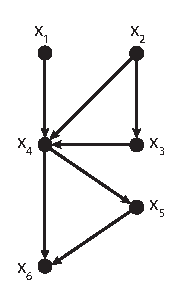
\includegraphics[]{resources/images/dependencias-condicionales}
	\caption{Dependencias condicionales}
	\label{fig:dependencias-condicionales}
\end{figure}

Por lo anterior, la estimación de la PDF conjunta se ha dividido en el producto de términos más sencillos.
En particular, Naïve Bayes es un caso especial en el que $A_i = \emptyset, i = 2, \ldots, l$

\subsection{Definición} 
\label{sec:definición}
Una red Bayesiana es un grafo acíclico dirigido (DAG) donde los nodos corresponden a variables aleatorias (las características).
Cada nodo es asociado con un conjunto de probabilidades condicionales, $P(x_i|A_i)$, donde $x_i$ es la variable asociada con el nodo específico y $A_i$ es el conjunto de sus padres en el grafo.

La especificación completa de una red bayesiana requiere el conocimiento de
\begin{enumerate*}
  \item Las probabilidades de los nodos raíz (aquellos sin un padre) y 
  \item Las probabilidades condicionales de los nodos no raiz, dados sus padres para todas las posibles combinaciones de sus valores.
\end{enumerate*}
La probabilidad conjunta es obtenida multiplicando todas las probabilidades condicionales con las probabilidades \emph{a priori} de los nodoz raíz.
Todo lo que se necesita es realizar un \emph{reordenamiento topológico} de las variables aleatorias, es decir, ordenar las variables de tal manera que cada variable aparece antes sus descendientes en el grafo relacionado.

\subsection{Aplicaciones} 
\label{sec:aplicaciones}
Las redes bayesianas han sido utilizadas en gran variedad de aplicaciones, especialmente en el diagnóstico médico.
La Figura~\ref{fig:ejemplo-red-bayesiana} muestra un ejemplo de su utilización.
La tabla del nodo raíz muestra la prevalencia de la enfermedad, es decir la frecuencia de que las personas sean fumadoras (\emph{probabilidad a priori}).
El resto de las tablas en cada uno de los nodos muestra las respectivas probabilidades condicionales.
\begin{figure}[h]
	\centering
	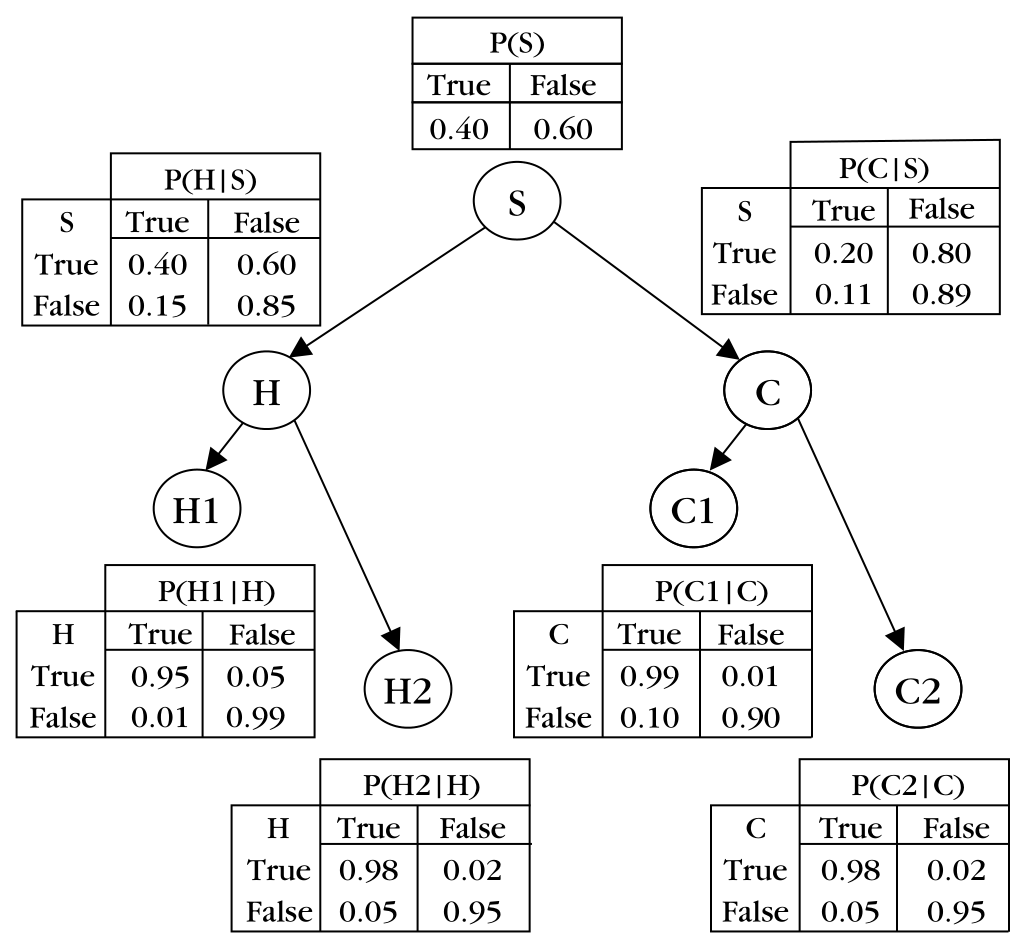
\includegraphics[scale=0.25]{resources/images/ejemplo-red-bayesiana}
	\caption{Red Bayesiana que modela las dependencias condicionales para fumadores (S) y sus tendencias para desarrollar cáncer (C) y enfermedades de corazón (H), junto a las variables correspondientes a pruebas de corazón (H1, H2) y exámenes de detección de cáncer (C1, C2)}
	\label{fig:ejemplo-red-bayesiana}
\end{figure}

Una vez que el DAG ha sido construido, la red bayesiana permite calcular eficientemente la probabilidad condicional de cualquier nodo en el grafo, dado que los valores de algunos de los otros nodos han sido observados.

\paragraph{Inferencia de probabilidad}
\label{par:inferencia_de_probabilidad}
La inferencia de probabilidad es la tarea más común que las redes bayesianas ayudan a solventar.
Conocidos los valores de algunas de las variables, llamados \emph{evidencia}, el objetivo es calcular las probabilidades condicionales para el resto de los valores de las variables.

Por ejemplo, dada la red Bayesiana mostrada en la Figura~\ref{fig:red-bayesiana-calculos}, a partir de los datos superiores (probabilidades a priori) es posible calcular las probabilidades condicionales mostradas en la parte inferior.
Nótese que por simplicidad no se utilizan subíndices, sino que las variables se denotan como $x,y,z,w$.
Asimismo, las variables son binarias y se utiliza el símbolo $x1$ cuando $x=1$ y $x0$ cuando $x=0$, haciendo lo mismo para el resto de variables.
Esta red bayesiana se encuentra completamente especificada por las probabilidades marginales del nodo raíz ($x$) y el resto de probabilidades condicionales de la parte superior.

\begin{figure}[h]
	\centering
	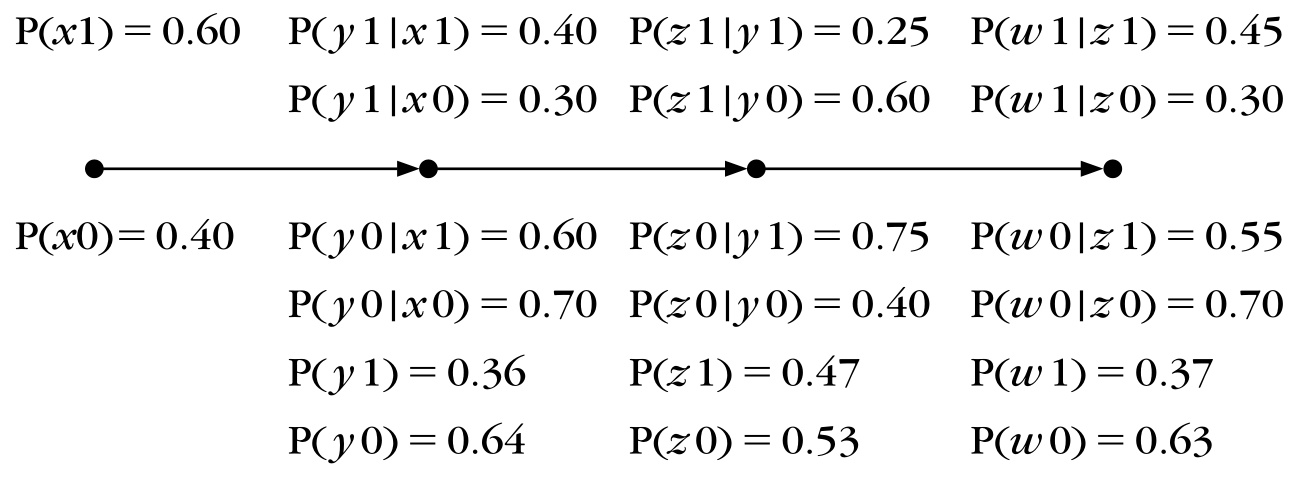
\includegraphics[scale=0.25]{resources/images/red-bayesiana-calculos}
	\caption{Red bayesiana con dependencias condicionales restringidas a una sola variable.}
	\label{fig:red-bayesiana-calculos}
\end{figure}

Así, tomando el nodo $y$ como ejemplo, es posible calcular sus probabilidades como:
\begin{eqnarray}
	p(y1) &=& p(y1 | x1)p(x1) + p(y1|x0)p(x0) = (0.4)(0.6) + (0.3)(0.4) = 0.36 \\
	p(y0) &=& 1-p(y1) = 0.64
\end{eqnarray}
Además, 
\begin{equation}
	p(y0 | x1) = 1 - p(y1 | x1)
\end{equation}
El resto de los valores puede ser calculado de forma similar.

Supongamos que se desea calcular 
\begin{enumerate*}[label=(\alph*)]
	\item $p(z1 | x1)$ y $p(w0 | x1)$ (habiendo medido $x$ y siendo su valor $x1$ como la evidencia), 
	\item $p(z1 | w1)$ (habiendo medido $w$ y siendo su valor $w1$ como la evidencia)
\end{enumerate*}

El cálculo de $p(z1 | x1)$ y $p(w0 | x1)$ puede ser realizado a través de:
\begin{eqnarray}
	p(z1 | x1) 	&=& p(z1 | y1,x1) p(y1|x1) + p(z1 | y0,x1) p(y0 | x1) \\
				&=& p(z1 | y1) p(y1|x1) + p(z1 | y0) p(y0 | x1) \\
				&=& (0.25)(0.4) + (0.6)(0.6) = 0.46 
\end{eqnarray}
y
\begin{eqnarray}
	p(w0 | x1) 	&=& p(w0 | z1,x1) p(z1|x1) + p(w0 | z0,x1) p(z0 | x1) \\
				&=& p(w0 | z1) p(z1|x1) + p(w0 | z0) p(z0 | x1) \\
				&=& (0.55)(0.46) + (0.7)(0.54) = 0.63
\end{eqnarray}

Para estos cálculos se observa una especie de algoritmo que pasa un mensaje (las probabilidades) hacia abajo ($x1$ es la evidencia), de un nodo hacia otro.

Para calcular $p(z1 | w1)$ la situación se invierte y ahora las probabilidades viajan hacia arriba ($w1$ es la evidencia).
\begin{equation}
	p(z1|w1) = \frac{p(w1|z1)p(z1)}{p(w1)} = \frac{(0.45)(0.47)}{0.37} = 0.57
\end{equation}

\paragraph{Entrenamiento de una red bayesiana} 
\label{par:entrenamiento_de_una_red_bayesiana}
El entrenamiento de una red bayesiana consiste en dos partes.
\begin{enumerate}
	\item Aprendizaje estructural: obtener la topología o estructura de la red.
	Esto puede ser realizado de forma externa con la asesoría de un experto, o bien siguiendo metodologías específicas de aprendizaje, las cuales se clasifican en:
	\begin{itemize}
		\item Aprendizaje de árboles.
		\item Aprendizaje de poliárboles.
		\item Aprendizaje de redes multiconectadas.
	\end{itemize}
	\item Aprendizaje paramétrico: Dada la estructura, obtener las probabilidades asociadas.
	Cuando se tienen datos completos y suficientes para todas las variables, el método más común es el estimador de máxima verosimilitud basado únicamente en las frecuencias de los datos.
	Cuando se carecen de datos suficientes, un método comúnmente elegido es el algoritmo de Expectation-Maximization (EM).
	Como ya ha sido observado, el algoritmo EM define los pasos:
	\begin{itemize}
		\item \textbf{Paso E}: se estiman los datos faltantes en base a los parámetros actuales.
		\item \textbf{Paso M}: Se estiman las probabilidades (parámetros) considerando los datos estimados.
	\end{itemize}
	De manera general, para los nodos ocultos en redes bayesianas, el algoritmo EM es el siguiente.
	\begin{enumerate}
		\item Iniciar los parámetros desconocidos (probabilidades condicionales) con valores aleatorios (o estimaciones de expertos).
		\item  Utilizar los datos conocidos con los parámetros actuales para estimar los valores de la variable(s) oculta(s).
		\item Utilizar los valores estimados para completar la tabla de datos.
		\item Re-estimar los parámetros con los nuevos datos.
		\item Repetir 2–4 hasta que no haya cambios significativos en las probabilidades.
	\end{enumerate}
\end{enumerate}


\section{Modelos Ocultos de Markov}
\label{sec:modelos_ocultos_de_markov_hidden_markov_models}
%http://www.comp.leeds.ac.uk/roger/HiddenMarkovModels/html_dev/main.html


\subsection{Introducción}
\label{sub:introducción}
En ocasiones, los datos a tratar provienen de escenarios en los que los componentes temporales juegan un papel primordial.
Así, surge el interés en encontrar patrones que ocurren a lo largo de secuencias temporales.
Por ejemplo, instrucciones solicitadas a una computadora, la secuencia de fonemas en palabras pronunciadas, o cualquier otra situación enfocada en eventos.

Considerar la siguiente situación.
Deducir el clima a partir de una alga marina.
Se conoce que un alga empapada significa un clima húmedo, mientras que un alga seca implica un clima soleado.
Si el alga está solamente húmeda, entonces existe un nivel de incertidumbre acerca del clima.
Naturalmente, el estado del clima no está restringido únicamente por el estado del alga; por ejemplo, el clima del día anterior representa una muy útil prueba para inferirlo.
Combinando el conocimiento disponible sobre el clima del día anterior y el estado del algo es posible obtener un mejor pronóstico para el clima de hoy.

\subsubsection*{Tipos de patrones}
\label{ssub:tipos_de_patrones}

\paragraph{Patrones deterministas} 
\label{par:patrones_determinísticos}
La secuencia de éstos puede ser descrita como una máquina de estados donde cada uno de ellos depende únicamene del estado previo: el sistema es determinista.
Por ejemplo, un semáforo (Figura ~\ref{fig:semaforo}).

\begin{figure}[]
	\centering
	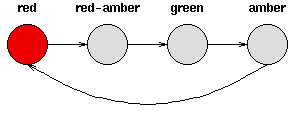
\includegraphics[]{resources/images/traffic-lights}
	\caption{Semáforo como fuente de patrones deterministas}
	\label{fig:semaforo}
\end{figure}

\paragraph{Patrones no deterministas}
\label{par:patrones_no_deterministas}
Los estados no mantienen una secuencia de forma determinista.
Aún así, es posible realizar una aproximación al sistema que genera dichos estados.

Por ejemplo, un modelo climatológico que defina los estados soleado, lluvioso y nublado es no determinista ya que no se puede indicar una secuencia específica y fija a través del tiempo para los estados.
Sin embargo, es posible asumir que el estado del modelo depende únicamente de sus estados previos; a esta consideración se le conoce como la \emph{propiedad de Markov} y se basa en la idea de que \emph{dado el presente, el pasado y el futuro son independientes}.
A través de dicha propiedad se simplifica la concepción del sistema pero también es posible causar pérdida de información.

\subsection{Proceso de Markov}
\label{sub:proceso_de_markov}
Un proceso de Markov es aquel que se mueve de un estado a otro dependiendo únicamente de los $n$ estados previos a lo largo de pasos de tiempo \textbf{discretos}.
El proceso es llamado de \emph{orden $n$} donde $n$ es el número de estados afectando la selección del siguiente estado.
El proceso de Markov más simple es uno de primer orden.
La diferencia respecto a un sistema determinista es que al selección es realizada de forma probabilística, no determinista.

La Figura~\ref{fig:transiciones-clima} muestra todas las posibles transiciones de primer orden entre los estados del ejemplo del clima.
Es importante notar que para un modelo de primer orden con $M$ estados existen $M^2$ trancisiones posibles.
\begin{figure}[h]
	\centering
	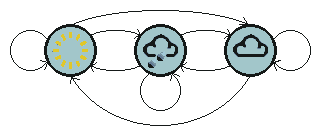
\includegraphics[scale=0.75]{resources/images/weather-example}
	\caption{Transiciones de primer orden en los estados del modelo climatológico}
	\label{fig:transiciones-clima}
\end{figure}

Para cada transición existe una probabilidad asociada conocida como probabilidad de transición de estado.
Las $M^2$ probabilidades conforman la \emph{matriz de transición de estados}.
La Figura~\ref{fig:matriz-transicion-clima} muestra un ejemplo de esta matriz.
Es importante notar que la suma de las probabilidades en cada renglón debe ser 1.
\begin{figure}[h]
	\centering
	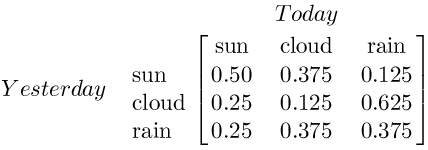
\includegraphics[scale=0.6]{resources/images/weather-matrix}
	\caption{Ejemplo de matriz de transición de estados}
	\label{fig:matriz-transicion-clima}
\end{figure}

Ahora bien, el sistema requiere definir un estado inicial, llamado el vector $\pi$.
Para el ejemplo del clima se debe indicar cuál era el clima en el día de la creación del modelo, como se muestra en la Figura~\ref{fig:vector-pi} (soleado).
\begin{figure}[tb]
	\centering
	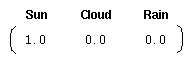
\includegraphics[]{resources/images/pi-vector}
	\caption{Vector pi (inicialización) del modelo del clima}
	\label{fig:vector-pi}
\end{figure}

De esta manera se ha definido un proceso de Markov mediante:
\begin{itemize}
	\item Un conjunto de estados \textbf{discretos} (soleado, nublado, lluvioso).
	\item Vector $\pi$ que define la probabilidad del sistema de encontrarse en cada estado en el tiempo $t_0$
	\item Matriz de transición de estados.
	Se asume que esta matriz no varía, sino que se mantiene fija a lo largo de la vida del sistema.
\end{itemize}

Cualquier sistema que pueda ser descrito a través de estos elementos califica para ser un proceso de Markov.

\subsection{Modelos ocultos de Markov (HMM)}
\label{sub:modelos_ocultos_de_markov}
En ocasiones los patrones que se desea encontrar no pueden ser descritos suficientemente por un proceso de Markov.

Retomando el ejemplo de averiguar el estado del clima mediante las algas, se conoce que ambos se encuentran relacionados.
Entonces se cuenta con dos conjuntos de estados, los estados observables (la situación del alga) y los estados ocultos (la situación del clima) que representan los estados VERDADEROS y que interesa conocer.
Entonces, lo que se busca es diseñar un algoritmo que permita predecir el clima a partir del estado del alga y asumiendo la premisa de Markov sin necesidad de ver directamente el estado del clima.

Un área de aplicación común de los HMM es el reconocimiento de voz en el que el sonido del habla es influido por diversos factores anatómicos.
La producción del lenguaje oral se considera como una secuencia de estados ocultos, y el sonido resultante como una secuencia de estados observables que en el mejor de los casos se aproxima al verdadero estado (el oculto).

Es importante notar que la cantidad de estados ocultos y los observables puede ser diferente.
En el ejemplo del clima, los estados ocultos son tres (soleado, nublado, lluvioso) mientras que los estados visibles son cuatro (el alga puede estar seca, secándose, húmeda o empapada).

Para estos casos la secuencia de estados observados se encuentra probabilísticamente relacionada con el proceso oculto.
Estos procesos se modelan utilizando un modelo oculto de Markov donde existe un proceso de Markov oculto evolucionando a lo largo del tiempo y un conjunto de estados observables que de alguna manera están relacionados con los estados ocultos.
Debido a esta anidación un HMM es también conocido como un \emph{proceso estocástico doblemente embebido}.
La Figura~\ref{fig:hmm-clima} muestra la representación gráfica del HMM del ejemplo del clima y las algas.

\begin{figure}[tb]
	\centering
	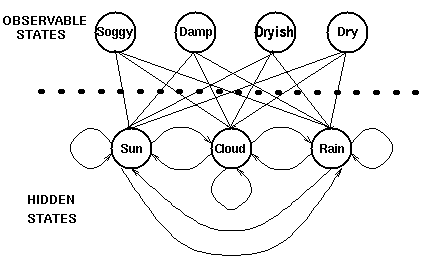
\includegraphics[scale=0.6]{resources/images/hidden-weather-example}
	\caption{HMM del ejemplo del clima y las algas}
	\label{fig:hmm-clima}
\end{figure}

Las conexiones entre estados ocultos y observables representan la probabilidad de generar un estado observado a partir de que el proceso de Markov se encuentre en un estado oculto en particular.
La suma de estas probabilidades que entran en un estado observable deberán sumar uno.
Para el caso del ejemplo es la suma de $p(Obs | Soleado), p(Obs | Nublado), p(Obs | Lluvioso)$.
En adición a las probabilidades que definen las transiciones entre estados en el proceso de Markov, se requiere otra matriz, llamada \emph{matriz de confusión}, que contiene las probabilidades de los estados observables dato un estado oculto en particular.
La Figura~\ref{fig:matriz-confusion} muestra la matriz de confusión para el ejemplo del clima.
\begin{figure}[tb]
	\centering
	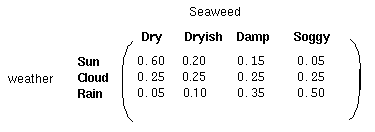
\includegraphics[scale=0.6]{resources/images/weather-confusion-matrix}
	\caption{Matriz de confusión del ejemplo del clima y las algas}
	\label{fig:matriz-confusion}
\end{figure}

\paragraph{Definición de un HMM} 
\label{par:definición_de_un_hmm}
Un HMM es una tripleta $(\pi,A,B)$ tal que
\begin{itemize}
	\item $\Pi = (\pi _i)$ es el vector de las probabilidades del estado inicial.
	\item $A = ( a_{ij})$ es la matriz de transición de estados, con las probabilidades $P(x_{i_{t}} | x_{j_{t-1}})$.
	\item $B = (b_{i_{j}})$ es la matriz de confusión, con las probabilidades $P(y_t | x_j)$
\end{itemize}
Las matrices de transición y confusión son independientes del tiempo y se mantienen fijas durante la evolución del sistema, lo cual representa la premisa más irrealizsta de lo modelos de Markov acerca de procesos del mundo real.

\subsection{Aplicaciones de los modelos ocultos de Markov}
\label{sub:aplicaciones_de_los_hmms}
Una vez que un sistema ha sido descrito a través de un HMM, tres problemas pueden ser solucionados.
Los dos primeros son problemas de reconocimiento de patrones, el tercero concierne a la generación de un HMM a partir de secuencias de observaciones.
A continuación se describen brevemente dichos problemas.

\paragraph{Evaluación} 
\label{par:evaluación}
Considérese el problema donde se cuenta con un número de HMMs (un conjunto de tripletas $(\pi,A,B)$) que describen diferentes sistemas y una secuencia de observaciones y que se desea conocer cuál de los HMM es más probable que haya generado la secuencia.
Por ejemplo, se podría contar con un modelo de \emph{verano} y otro para \emph{invierno} para el alga dado que su comportamiento varía de estación a estación.

Para este problema, se ha utilizado el algoritmo \emph{forward} para calcular dicha probabilidad.
Este tipo de problema ocurre a menudo en sistemas de reconocimiento del habla donde un gran número de modelos de Markov serán utilizados, cada uno modelando una palabra en particular.
Entonces, a partir de la pronunciación de una palabra se crea una secuencia de observación y la palabra es reconocida al identificar cuál es el HMM más probable según su pronunciación.

\paragraph{Decodificación} 
\label{par:decodificación}
\emph{Encontrar la secuencia más probable de estados ocultos dado un conjunto de observaciones}.
Este problema resulta interesante ya que los estados ocultos son los que contienen la información real que representa \emph{algo} en el mundo real.

El ejemplo del clima y las algas pertenece a este problema, ya que a partir del estado del alga (estado visible) se desea conocer el clima (estado invisible).

El algoritmo \emph{Viterbi} es el más utilizado para determinar la secuencia de estados ocultos más probables, dada una secuencia de observaciones y un HMM.

Un uso ampliamente difundido del algoritmo Viterbi se encuentra en el Procesamiento de Lenguaje Natural, para etiquetar palabras de acuerdo a su clase sintáctica (verbo, sustantivo, etc).
Las palabras en una oración son los estados observables y las cláses sintácticas son los estados ocultos.
Al encontrar los estados ocultos mas probables para una oración, se habrán encontrado las clases sintácticas más probables para una palabra dado su contexto.

\paragraph{Aprendizaje}
\label{par:aprendizaje}
\emph{Generar un HMM a partir de una secuencia de observaciones}.
Consiste en tomar una secuencia de observaciones (de un conjunto conocido) que se sabe que representa a un conjunto de estados ocultos y obtener el HMM más probable.
Es decir, determinar la tripleta $(\pi,A,B)$ que tiene la mayor probabilidad de describir lo que ha visto.,
El algoritmo \emph{forward-backward} es el más utilizado para realizar esta labor.

\newpage 
\nocite{*}
\bibliographystyle{natdin}
\bibliography{references} 

\end{document}